% This is part of Un soupçon de mathématique sans être agressif pour autant
% Copyright (c) 2014-2015
%   Laurent Claessens
% See the file fdl-1.3.txt for copying conditions.

% This is part of Un soupçon de mathématique sans être agressif pour autant
% Copyright (c) 2014-2015
%   Laurent Claessens
% See the file fdl-1.3.txt for copying conditions.

On croise deux bandes de papier et on s'intéresse à l'intersection.  Quels quadrilatères peut-on obtenir ?
\begin{center}
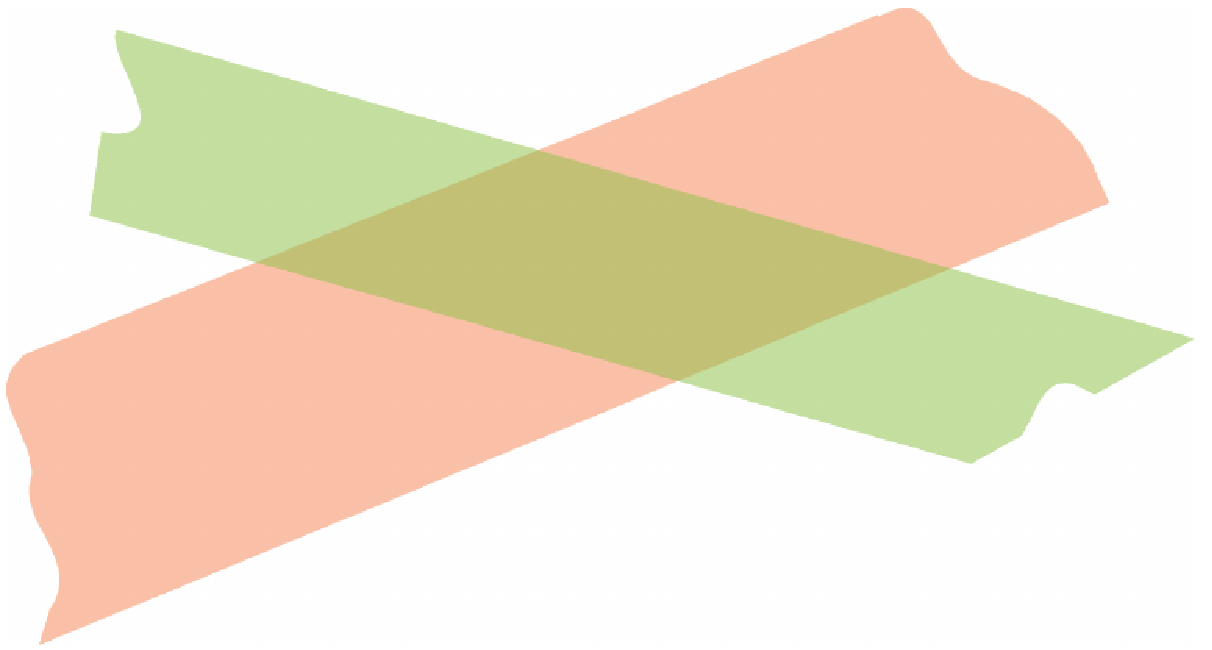
\includegraphics[width=5cm]{deux_bandes.pdf}
\end{center}

De \cite{NRHooXFvgpp5}

%+++++++++++++++++++++++++++++++++++++++++++++++++++++++++++++++++++++++++++++++++++++++++++++++++++++++++++++++++++++++++++ 
\section{Définitions et propriétés}
%+++++++++++++++++++++++++++++++++++++++++++++++++++++++++++++++++++++++++++++++++++++++++++++++++++++++++++++++++++++++++++ 

Le but de cette section est de donner les définitions des principaux quadrilatères et de montrer que «tout le reste» sont des propriétés à démontrer.
\begin{definition}
    Quelque quadrilatères :
    \begin{enumerate}
        \item
            Un \defe{parallélogramme}{parallélogramme} est un quadrilatère qui a ses côtés opposés parallèles deux à deux.
        \item
            Un \defe{losange}{losange} est un quadrilatère qui possède quatre côtés de même longueur.
        \item
            Un \defe{rectangle}{rectangle} est un quadrilatère qui a quatre angles droits.
        \item
            Un \defe{carré}{carré} est un rectangle qui a ses côtés de même longueur.
    \end{enumerate}
\end{definition}

\begin{propriete}
    Les diagonales d'un carré sont perpendiculaires.
\end{propriete}

\begin{proof}
    Dessinons un carré :
    \begin{center}
        \input{Fig_UOEOooLxhpSC.pstricks}
    \end{center}
    Par définition un carré a ses côtés de même longueurs, donc le triangle \( ADC\) est isocèle en \( D\).
    \begin{center}
        Donc \( a_1=c_2\)
    \end{center}
    Mais comme la somme des angles internes du triangle doit faire \SI{180}{\degree} et que l'angle \( \hat D\) en fait \( 90\), 
    \begin{center}
        \( a_1=a_2=\SI{45}{\degree}\).
    \end{center}
    Le même raisonnement dans les triangles \( ABC\), \( ADB\) et \( CDB\) donne :
    \begin{equation}
        a_1=a_2=b_1=b_2=c_1=c_2=d_1=d_2=\SI{45}{\degree}.
    \end{equation}
    
    Dans le triangle \( DCI\), la somme des angles doit faire \SI{180}{\degree}. Mais les deux angles de base font \SI{45}{\degree}. Donc le troisième angle doit mesurer \SI{90}{\degree}.

\end{proof}

% This is part of Un soupçon de mathématique sans être agressif pour autant
% Copyright (c) 2015
%   Laurent Claessens
% See the file fdl-1.3.txt for copying conditions.

%--------------------------------------------------------------------------------------------------------------------------- 
\subsection*{Activité : symétries dans les quadrilatères}
%---------------------------------------------------------------------------------------------------------------------------

Donner les éventuels centres et axes de symétrie des figures suivantes :
\begin{multicols}{2}
\begin{enumerate}
    \item
\input{Fig_ENQZooVqRaIv0.pstricks}
    \item
\input{Fig_ENQZooVqRaIv1.pstricks}
    \item
\input{Fig_ENQZooVqRaIv2.pstricks}
    \item
\input{Fig_ENQZooVqRaIv3.pstricks}
\end{enumerate}
\end{multicols}




%+++++++++++++++++++++++++++++++++++++++++++++++++++++++++++++++++++++++++++++++++++++++++++++++++++++++++++++++++++++++++++ 
\section{Diagonales}
%+++++++++++++++++++++++++++++++++++++++++++++++++++++++++++++++++++++++++++++++++++++++++++++++++++++++++++++++++++++++++++

\begin{propriete}
    Si deux droites sont coupées par une droite de telle sorte que les angles alternes-internes soient égaux alors les deux droites sont parallèles.
\end{propriete}

\begin{center}
\input{Fig_QEPZooNndwiS.pstricks}
\end{center}


\begin{propriete}
    \begin{enumerate}
        \item
            Les côtés opposés d'un parallélogramme sont de même longueurs.
        \item
            Les angles opposés d'un parallélogramme ont même mesure.
    \end{enumerate}
\end{propriete}

\begin{proof}
    Dans le parallélogramme \( ABCD\) nous traçons la diagonale et nous considérons les angles\ldots

\begin{center}
   \input{Fig_ZUVLooJNWbPB0.pstricks}
\end{center}

    Les droites \( (DA)\) et \( (CB)\) sont parallèles (parce qu'on a un parallélogramme), donc les angles \( a_1\) et \( c_2\) sont alternes-internes et donc égaux.

    De la même façon, les angles \( a_2\) et \( c_1\) sont égaux parce qu'alternes-internes aux droites parallèles \( (DC)\) et \( (AB)\).

    Voici la situation actuelle :
    \begin{center}
        \input{Fig_ZUVLooJNWbPB1.pstricks}
    \end{center}
    Maintenant les triangles \( CAD\) et \( ACB\) sont égaux parce qu'ils ont deux angles égaux et un côté en commun. Nous en déduisons que les toutes les autres longueurs et angles de ces deux triangles sont égales :
    \begin{equation}
        CB=DA
    \end{equation}
    et
    \begin{equation}
        DC=AB,
    \end{equation}
    et
    \begin{equation}
     \widehat{CDA}=\widehat{ABC},
    \end{equation}
    ce qu'il fallait démontrer.
\end{proof}

\begin{propriete}
    \begin{enumerate}
        \item
            Un quadrilatère est une parallélogramme si et seulement si ses deux diagonales se coupent en leur milieu.
        \item
            Le centre d'un parallélogramme est centre de symétrie.
    \end{enumerate}
\end{propriete}


\begin{center}
   \input{Fig_TFDNooJemFMW.pstricks}
\end{center}


